Network designers need to gather analytics about the performance of the network to better understand what is happening behind the curtain. 
\ingreen{These are useful for traffic engineering, 
for reaching a higher utilization of the infrastructure,
for reducing link congestion, and for detecting anomalies when they happen.} Switches generally do not have sufficient memory to hold entire measurement models for large data streams, therefore the network designer generally sacrifices accuracy for a lower memory footprint.
Data sketching algorithms, or \textit{sketches} for short \cite{cormode2012synopses}, are
an indispensable tool for such high-speed low-memory-footprint computations. Sketches  estimate some function
of a large stream \ingreen{such as} \inblue{flow sizes}~\cite{CountMin} (i.e., the number of packets in a flow), \inblue{stream cardinality}~\cite{datar2002comparing, flajolet1983probabilistic} (i.e., the number of flows in a stream), the top-$k$ most common items~\cite{metwally2005efficient} or  frequency changes~\cite{IMCBal03}.
They are supported by many data analytics platforms such as PowerDrill~\cite{heule2013hyperloglog},
Druid~\cite{druid}, Hillview~\cite{hillview}, and Presto~\cite{presto} as well as \ingreen{by} standalone toolkits~\cite{apache-datasketches}.


Measurements are conducted in switches  all over the network; however, to successfully analyze network behavior, measurement data needs to be gathered in a centralized server that can see \ingreen{a wider view}.
\forRevThree{A stream of multiple flows passes through the network, with disjoint parts of the stream sampled by multiple \emph{ingestion nodes}, where parts of the same flow may be ingested by different nodes. The ingestion nodes periodically propagate their local sketch to a \emph{central node}, as illustrated in Figure~\ref{sktc-fig:ingestion-nodes}.  The network has to handle the trade-off of sending data packets vs. sending crucial control packets with sketch information~\cite{zhang2010optimizing, %zhang2009spatio,
benson2010understanding}. A way to reduce these control packets is by compressing the sketches before transferring them to a central analytics node.}



%\inred{To capture this behavior, we treat all of the incoming packets to the network as originating from a single \emph{stream}, which consists of multiple \emph{flows}.}
%\inblue{The stream is split into disjoint parts observed by multiple \emph{ingestion nodes}. Parts of the same flow may be ingested by different nodes.}  Once the nodes have a sketch ready to be sent (e.g., they periodically receive a packet signaling the end of their current stream and start a new one) they propagate their local sketch to a \emph{central node}~\cite{huang2017sketchvisor, li2016flowradar, liu2016one}. This is illustrated in Figure~\ref{sktc-fig:ingestion-nodes}. The network has to handle the trade-off of sending data packets vs. sending crucial control packets~\cite{zhang2010optimizing, %zhang2009spatio,
%benson2010understanding} with sketch information. A way to reduce these control packets is by compressing the sketches before transferring them to a central analytics node. 

\inblue{Compressing is crucial as network managers may have many sketches estimating different measurements concurrently. While each sketch alone may be insignificant, their aggregate is noticeable at the network level. Additionally, the sketch may be collecting measurements in low bandwidth networks~\cite{muthitacharoen2001low, margaritis2003peer}}, \ingreen{making the sketch size critical.}


\begin{figure}
    \centering
    %\includegraphics[width=0.9\linewidth]{figures/IngestionNodesPic.png}
    \tikzset{every picture/.style={line width=0.75pt}} %set default line width to 0.75pt    
    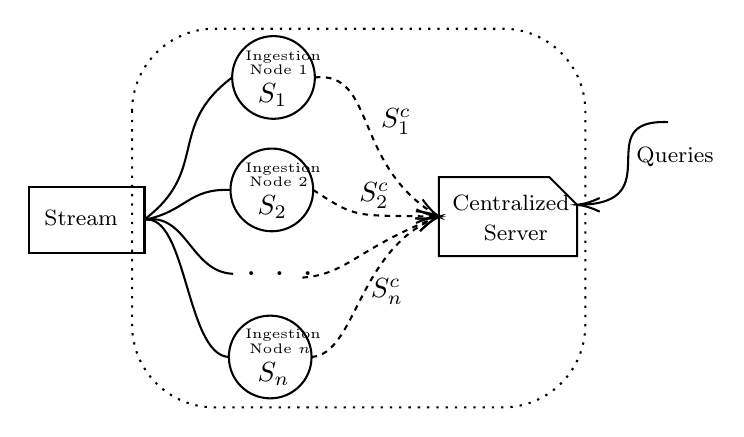
\begin{tikzpicture}[x=0.75pt,y=0.75pt,yscale=-1,xscale=1]
    %uncomment if require: \path (0,300); %set diagram left start at 0, and has height of 300
    
    %Shape: Rectangle [id:dp7800934124171983] 
    \draw   (117,155.65) -- (172.78,155.65) -- (172.78,187.53) -- (117,187.53) -- cycle ;
    %Shape: Ellipse [id:dp20814509523202052] 
    \draw   (215.02,103.05) .. controls (215.02,92.05) and (223.94,83.13) .. (234.94,83.13) .. controls (245.95,83.13) and (254.87,92.05) .. (254.87,103.05) .. controls (254.87,114.06) and (245.95,122.98) .. (234.94,122.98) .. controls (223.94,122.98) and (215.02,114.06) .. (215.02,103.05) -- cycle ;
    %Shape: Ellipse [id:dp5192677502317808] 
    \draw   (214.22,157.24) .. controls (214.22,146.24) and (223.14,137.32) .. (234.15,137.32) .. controls (245.15,137.32) and (254.07,146.24) .. (254.07,157.24) .. controls (254.07,168.25) and (245.15,177.17) .. (234.15,177.17) .. controls (223.14,177.17) and (214.22,168.25) .. (214.22,157.24) -- cycle ;
    %Shape: Circle [id:dp7676828342293531] 
    \draw   (213.43,237.73) .. controls (213.43,226.73) and (222.35,217.81) .. (233.35,217.81) .. controls (244.35,217.81) and (253.27,226.73) .. (253.27,237.73) .. controls (253.27,248.74) and (244.35,257.66) .. (233.35,257.66) .. controls (222.35,257.66) and (213.43,248.74) .. (213.43,237.73) -- cycle ;
    %Snip Single Corner Rect [id:dp7350487709437881] 
    \draw   (314.63,151.1) -- (367.87,151.1) -- (381.18,164.41) -- (381.18,189.12) -- (314.63,189.12) -- cycle ;
    %Curve Lines [id:da7243599111171348] 
    \draw   [dash pattern={on 2pt off 2pt}]   (254.87,103.05) .. controls (284.45,99.9) and (273.03,145.17) .. (313.4,169.38) ;
    \draw [shift={(314.63,170.11)}, rotate = 209.86] [color={rgb, 255:red, 0; green, 0; blue, 0 }  ][line width=0.75]    (10.93,-3.29) .. controls (6.95,-1.4) and (3.31,-0.3) .. (0,0) .. controls (3.31,0.3) and (6.95,1.4) .. (10.93,3.29)   ;
    %Curve Lines [id:da4335557046839309] 
    \draw   [dash pattern={on 2pt off 2pt}]   (254.07,157.24) .. controls (275.66,171.37) and (273.66,169.27) .. (312.82,170.07) ;
    \draw [shift={(314.63,170.11)}, rotate = 181.27] [color={rgb, 255:red, 0; green, 0; blue, 0 }  ][line width=0.75]    (10.93,-3.29) .. controls (6.95,-1.4) and (3.31,-0.3) .. (0,0) .. controls (3.31,0.3) and (6.95,1.4) .. (10.93,3.29)   ;
    %Curve Lines [id:da47273415849462186] 
    \draw   [dash pattern={on 2pt off 2pt}]   (253.27,237.73) .. controls (274.86,236.16) and (275.18,186.66) .. (312.89,170.81) ;
    \draw [shift={(314.63,170.11)}, rotate = 519.15] [color={rgb, 255:red, 0; green, 0; blue, 0 }  ][line width=0.75]    (10.93,-3.29) .. controls (6.95,-1.4) and (3.31,-0.3) .. (0,0) .. controls (3.31,0.3) and (6.95,1.4) .. (10.93,3.29)   ;
    %Curve Lines [id:da7986835200568454] 
    \draw   [dash pattern={on 2pt off 2pt}]   (248.89,199.48) .. controls (270.48,197.91) and (275.05,185.52) .. (312.88,170.78) ;
    \draw [shift={(314.63,170.11)}, rotate = 519.15] [color={rgb, 255:red, 0; green, 0; blue, 0 }  ][line width=0.75]    (10.93,-3.29) .. controls (6.95,-1.4) and (3.31,-0.3) .. (0,0) .. controls (3.31,0.3) and (6.95,1.4) .. (10.93,3.29)   ;
    %Rounded Rect [id:dp16891083296577403] 
    \draw  [dash pattern={on 0.84pt off 2.51pt}] 
    (166.81,119.26) .. controls (166.81,97.34) and (184.58,79.57) .. (206.49,79.57) -- (345.47,79.57) .. controls (367.39,79.57) and (385.16,97.34) .. (385.16,119.26) -- 
    %(166.81,113.26) .. controls (166.81,91.34) and (184.58,73.57) .. (206.49,73.57) -- (345.47,73.57) .. controls (367.39,73.57) and (385.16,91.34) .. (385.16,113.26) -- 
    %(385.16,232.31) .. controls (385.16,254.23) and (367.39,272) .. (345.47,272) -- (206.49,272) .. controls (184.58,272) and (166.81,254.23) .. (166.81,232.31) -- cycle ;
    (385.16,222.31) .. controls (385.16,244.23) and (367.39,262) .. (345.47,262) -- (206.49,262) .. controls (184.58,262) and (166.81,244.23) .. (166.81,222.31) -- cycle ;
    
    %Curve Lines [id:da7483451131891823] 
    \draw    (172.5,171.67) .. controls (204.38,147.76) and (183.14,126.96) .. (215.02,103.05) ;
    %Curve Lines [id:da3567735385248336] 
    \draw    (172.5,171.67) .. controls (193.22,167.68) and (193.5,156.45) .. (214.22,157.24) ;
    %Curve Lines [id:da8413889792937872] 
    \draw    (172.5,171.67) .. controls (193.22,167.68) and (194.78,196.87) .. (215.5,197.67) ;
    %Curve Lines [id:da820436037263437] 
    \draw    (172.5,171.67) .. controls (193.22,167.68) and (192.71,236.94) .. (213.43,237.73) ;
    %Curve Lines [id:da6059682612620094] 
    \draw    (425.01,124.57) .. controls (386.35,122.99) and (426.58,163.59) .. (382.54,164.39) ;
    \draw [shift={(381.18,164.41)}, rotate = 360.01] [color={rgb, 255:red, 0; green, 0; blue, 0 }  ][line width=0.75]    (10.93,-3.29) .. controls (6.95,-1.4) and (3.31,-0.3) .. (0,0) .. controls (3.31,0.3) and (6.95,1.4) .. (10.93,3.29)   ;
    
    % Text Node
    \draw (123.1,165.49) node [anchor=north west][inner sep=0.75pt]  [font=\footnotesize] [align=left] {Stream};
    % Text Node
    \draw (219.94,88.66) node [anchor=north west][inner sep=0.75pt]   [align=left] {{\tiny Ingestion}};
    \draw (221.94,95.66) node [anchor=north west][inner sep=0.75pt]   [align=left] {{\tiny Node 1}};
    \draw (225.94,104.66) node [anchor=north west][inner sep=0.75pt]   [align=left] {\textit{$S_1$}};
    % Text Node
    \draw (219.84,142.65) node [anchor=north west][inner sep=0.75pt]   [align=left] {{\tiny Ingestion }};
    \draw (221.84,149.65) node [anchor=north west][inner sep=0.75pt]   [align=left] {{\tiny Node 2}};
    \draw (225.84,158.55) node [anchor=north west][inner sep=0.75pt]   [align=left] {\textit{$S_2$}};
    % Text Node
    \draw (219.84,222.73) node [anchor=north west][inner sep=0.75pt]   [align=left] {{\tiny Ingestion }};
    \draw (221.84,229.73) node [anchor=north west][inner sep=0.75pt]   [align=left] {{\tiny Node $n$}};
    \draw (225.84,238.73) node [anchor=north west][inner sep=0.75pt]   [align=left] {\textit{$S_n$}};
    % Text Node
    \draw (319.63,158.1) node [anchor=north west][inner sep=0.75pt]  [font=\small] [align=left] {{\footnotesize Centralized }\\{\footnotesize  \ \ \ \ Server}};
    % Text Node
    \draw (285.31,116.67) node [anchor=north west][inner sep=0.75pt]   [align=left] {\textit{$S^c_1$}};%{\textit{S{\tiny 1}}};
    % Text Node
    \draw (274.76,152.33) node [anchor=north west][inner sep=0.75pt]   [align=left] {\textit{$S^c_2$}};
    % Text Node
    \draw (280.34,198.55) node [anchor=north west][inner sep=0.75pt]   [align=left] {\textit{$S^c_n$}};
    % Text Node
    \draw (220.15,195.31) node [anchor=north west][inner sep=0.75pt]   [align=left] {{\Large . . .}};
    % Text Node
    \draw (408.29,135.38) node [anchor=north west][inner sep=0.75pt]  [font=\footnotesize] [align=left] {Queries};
    
    \end{tikzpicture}
    \caption{Network-wide measurement over $n$ ingestion nodes: Queries are answered by  a centralized server collecting summaries $S^c_1, \ldots, S^c_n$ of the local sketches $S_1, \ldots, S_n$ (e.g., the Count-Min sketch (CM) or the K-minimum-values (KMV) sketch) in the ingestion nodes.}
    \label{sktc-fig:ingestion-nodes}
\end{figure}

A framework for sketch compression was suggested by Yang et al.~\cite{yang2018elastic}. A major component of this framework, named \emph{Maximum Merging Algorithm (\textbf{MM})}, compresses a Count-Min sketch (CM) by utilizing a $\max$ function and merging multiple cells in one CM to generate a new, smaller sketch. 
The first limitation of that approach is that it compresses a sketch only into smaller sketches of particular sizes, those that have a common divisor with the size of the original sketch. Moreover, the approach does not provide insights for the selection of the various compression ratios that should be implied for a distributed measurement in multiple nodes. In particular, how the traffic distribution among the nodes should be considered. 
%However, this compression method has two issues we attempt to resolve.  We allow higher flexibility and propose a new method called CM-SKTC that supports compressing a CM to any size needed sketch. Our second contribution is that we suggest a traffic-aware compression method that considers the distribution among the ingestion nodes and allocates to each node the summary size it should report, such that a node that received a larger portion of the traffic sends a larger summary and vice versa.
 
A clear drawback of compression methods is the accuracy reduction they might imply. 
%However network managers want to have data that has some guarantees of its accuracy. 
It is often critical for network managers to have access to measurements with guarantees of their accuracy.
In the common case that the network has multiple ingestion nodes that generate the measurements and send the data to a centralized server, it is intuitive to allow each node to report them through an amount of data that is correlative to the amount of traffic it observes. In this paper,  \emph{we study distributed sketch-based network measurement with limited communication. For optimizing accuracy  we call for traffic-aware compression ratios of the multiple sketch instances.} We present a formal model that refers to any given number of ingestion nodes and any distribution of the traffic through these nodes. Moreover, the resize factors also guarantee that the amount of data  sent over the network is less than compressing all the data from all the nodes to the same size with previously presented methods.




We present the following major contributions: 

%\emph{(i)} We motivate a compression method for distributed measurement which is traffic aware. We focus on the CM and describe the traffic-aware Count-Min sketch, denoted TA-CM, that computes the ideal compression ratios for the various nodes for reducing the total amount of reported data. We provide guarantees on the error bounds of the approach.
\emph{(i)} As a building block, we develop a compression method named CM-SKTC for a single CM that allows general compression ratios, and then present the Traffic-Aware CM sketch, denoted TA-CM.



\emph{(ii)} We present Traffic-Aware K-minimum-values (KMV), denoted TA-KMV -- a traffic-aware compression ratio for nodes implementing distributed distinct flow count with the KMV sketch.

\inblue{
\emph{(iii)} Finally, we present Traffic-Aware HyperLogLog (HLL), denoted TA-HLL -- a traffic-aware compression ratio for nodes implementing distributed distinct flow count with the HLL sketch.
}


%\inblue{
%A preliminary version of this article %\inred{appeared} at IFIP Networking, Virtual %Conference, June 2021~\cite{IFIP21}. This submission %includes the following new technical contributions:}

%\inblue{
%(i) The proofs for Lemma 1 and Theorems 1 and 2 are %first presented here. Lemma 2 and its proof is also %first presented here.}

%\inblue{
%(ii) An extension of the traffic-aware approach to %the HyperLogLog sketch (Section II.C and Section %VI). Experimental results for this sketch appear in %the Section VII.E. 
%}

The rest of the paper is organized as follows. Section \ref{sktc-sec:background} discusses \forRevThree{preliminaries, our model,} and related work. In Section \ref{sktc-sec:com-sketch} we present the CM-SKTC compression method for a single CM, bound its error, and describe how to decrease the data sent from ingestion nodes to the centralized server. 
The TA-CM for traffic-aware CM compression for multiple nodes is described in Section~\ref{sktc-sec:resize}.  
Section~\ref{sktc-sec:kmv-sktc} presents the TA-KMV for cardinality estimation (count distinct). Experimental evaluation of the methods is provided in Section \ref{sktc-sec:evaluation}. Finally, in Section \ref{sktc-sec:conclusion} we conclude and suggest directions for future work.